%%%%%%%%%%%%%%%%%%%%%%%%%%%%%%%%%%%%%%%%%%%%%%
%                insertmeeting
% 1) Title (something creative & funny?)
% 2) Date (MM/DD/YYYY)
% 3) Location (ex. Hagerty High School)
% 4) People/Committees Present 
% 5) Picture 
% 6) Start Time & Stop Time (ex. 12:30AM to 4:30PM)
%%%%%%%%%%%%%%%%%%%%%%%%%%%%%%%%%%%%%%%%%%%%%%
\insertmeeting 
	{Intake Assemble!} 
	{12/30/21} 
	{Hagerty High School}
	{Jensen}
	{Images/RobotPics/robot.jpg}
	{2:30 - 4:30}
	
\hhscommittee{Hardware}
\noindent\hfil\rule{\textwidth}{.4pt}\hfil
\subsubsection*{Goals}
\begin{itemize}
    \item Build and test new roller intake

\end{itemize} 

\noindent\hfil\rule{\textwidth}{.4pt}\hfil

\subsubsection*{Accomplishments}
After waiting for all of the parts to print for the roller intake, we are ready to assemble it and do some testing to see if it will work. To start off the meeting, we pressed all of the shafts into our PLA pulleys. These were printed on a lower quality printer because of their low likelihood of breaking and to decrease the wait time for 3D printed parts. The parts we are using are belts and pulleys (XL and O-ring),bearings, hex shafts, a roller, a graphite pole, the base of the intake, and the roller arm (Figure \ref{fig:123021_1}). The 3d printed intake base, which we added pockets to to reduce weight, ended up weighing just 39 grams, an improvement of almost 20 grams from the previous, unpocketed version (Figure \ref{fig:123021_2}). We started putting all of the parts together just as we had designed them in CAD. Because we didn’t have any surgical tubing on hand because we were working at UCF, we covered the roller in rubber bands which made a good enough substitute (Figure \ref{fig:123021_3}). 
With the intake complete (Figure \ref{fig:123021_4}), we moved onto testing. Although we don't yet have a mount for the servo that powers the entire intake, we still wanted to try the intake to see if the idea worked at all. Connecting a drill to one of the shafts, we spun the intake at a speed that seemed similar to a superspeed servo, which is what we plan to use on the final intake (Figure \ref{fig:123021_5}). While intaking and out-taking, the intake worked very nicely, easily and quickly sucking the blocks in with little effort. Using a spring to tension the roller arm downwards allowed the intake to adapt to the different sized balls and cubes, working flawlessly, just as we had designed it to. Even while out-taking, the intake was able to release the elements without shooting them out, which was our main concern with the design (Figure \ref{fig:123021_6}). Feeling fulfilled and proud with our intake design, we started discussing weather it would be ready for competition next week. Although this intake looked promising, it still used a graphite pole, which doesn't have a fully complete design yet, and it lacks a servo mount or any belt to connect the servo to the intake. Still this design working is a massive step in the right direction in terms of design, proving the concept can work as we want it to.
 

\begin{figure}[ht]
\centering
\begin{minipage}[b]{.48\textwidth}
  \centering
  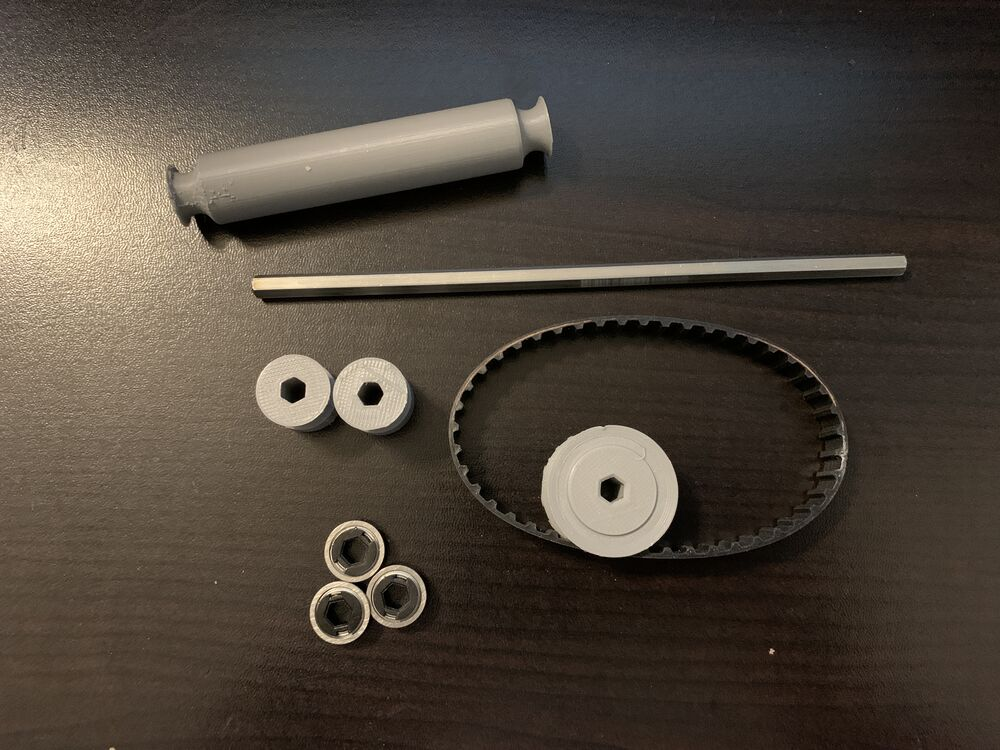
\includegraphics[width=0.95\textwidth]{Meetings/December/12-30-21/12-30-21_Hardware_Figure1 - Nathan Forrer.JPG}
  \caption{Our intake parts}
  \label{fig:123021_1}
\end{minipage}%
\hfill%
\begin{minipage}[b]{.48\textwidth}
  \centering
  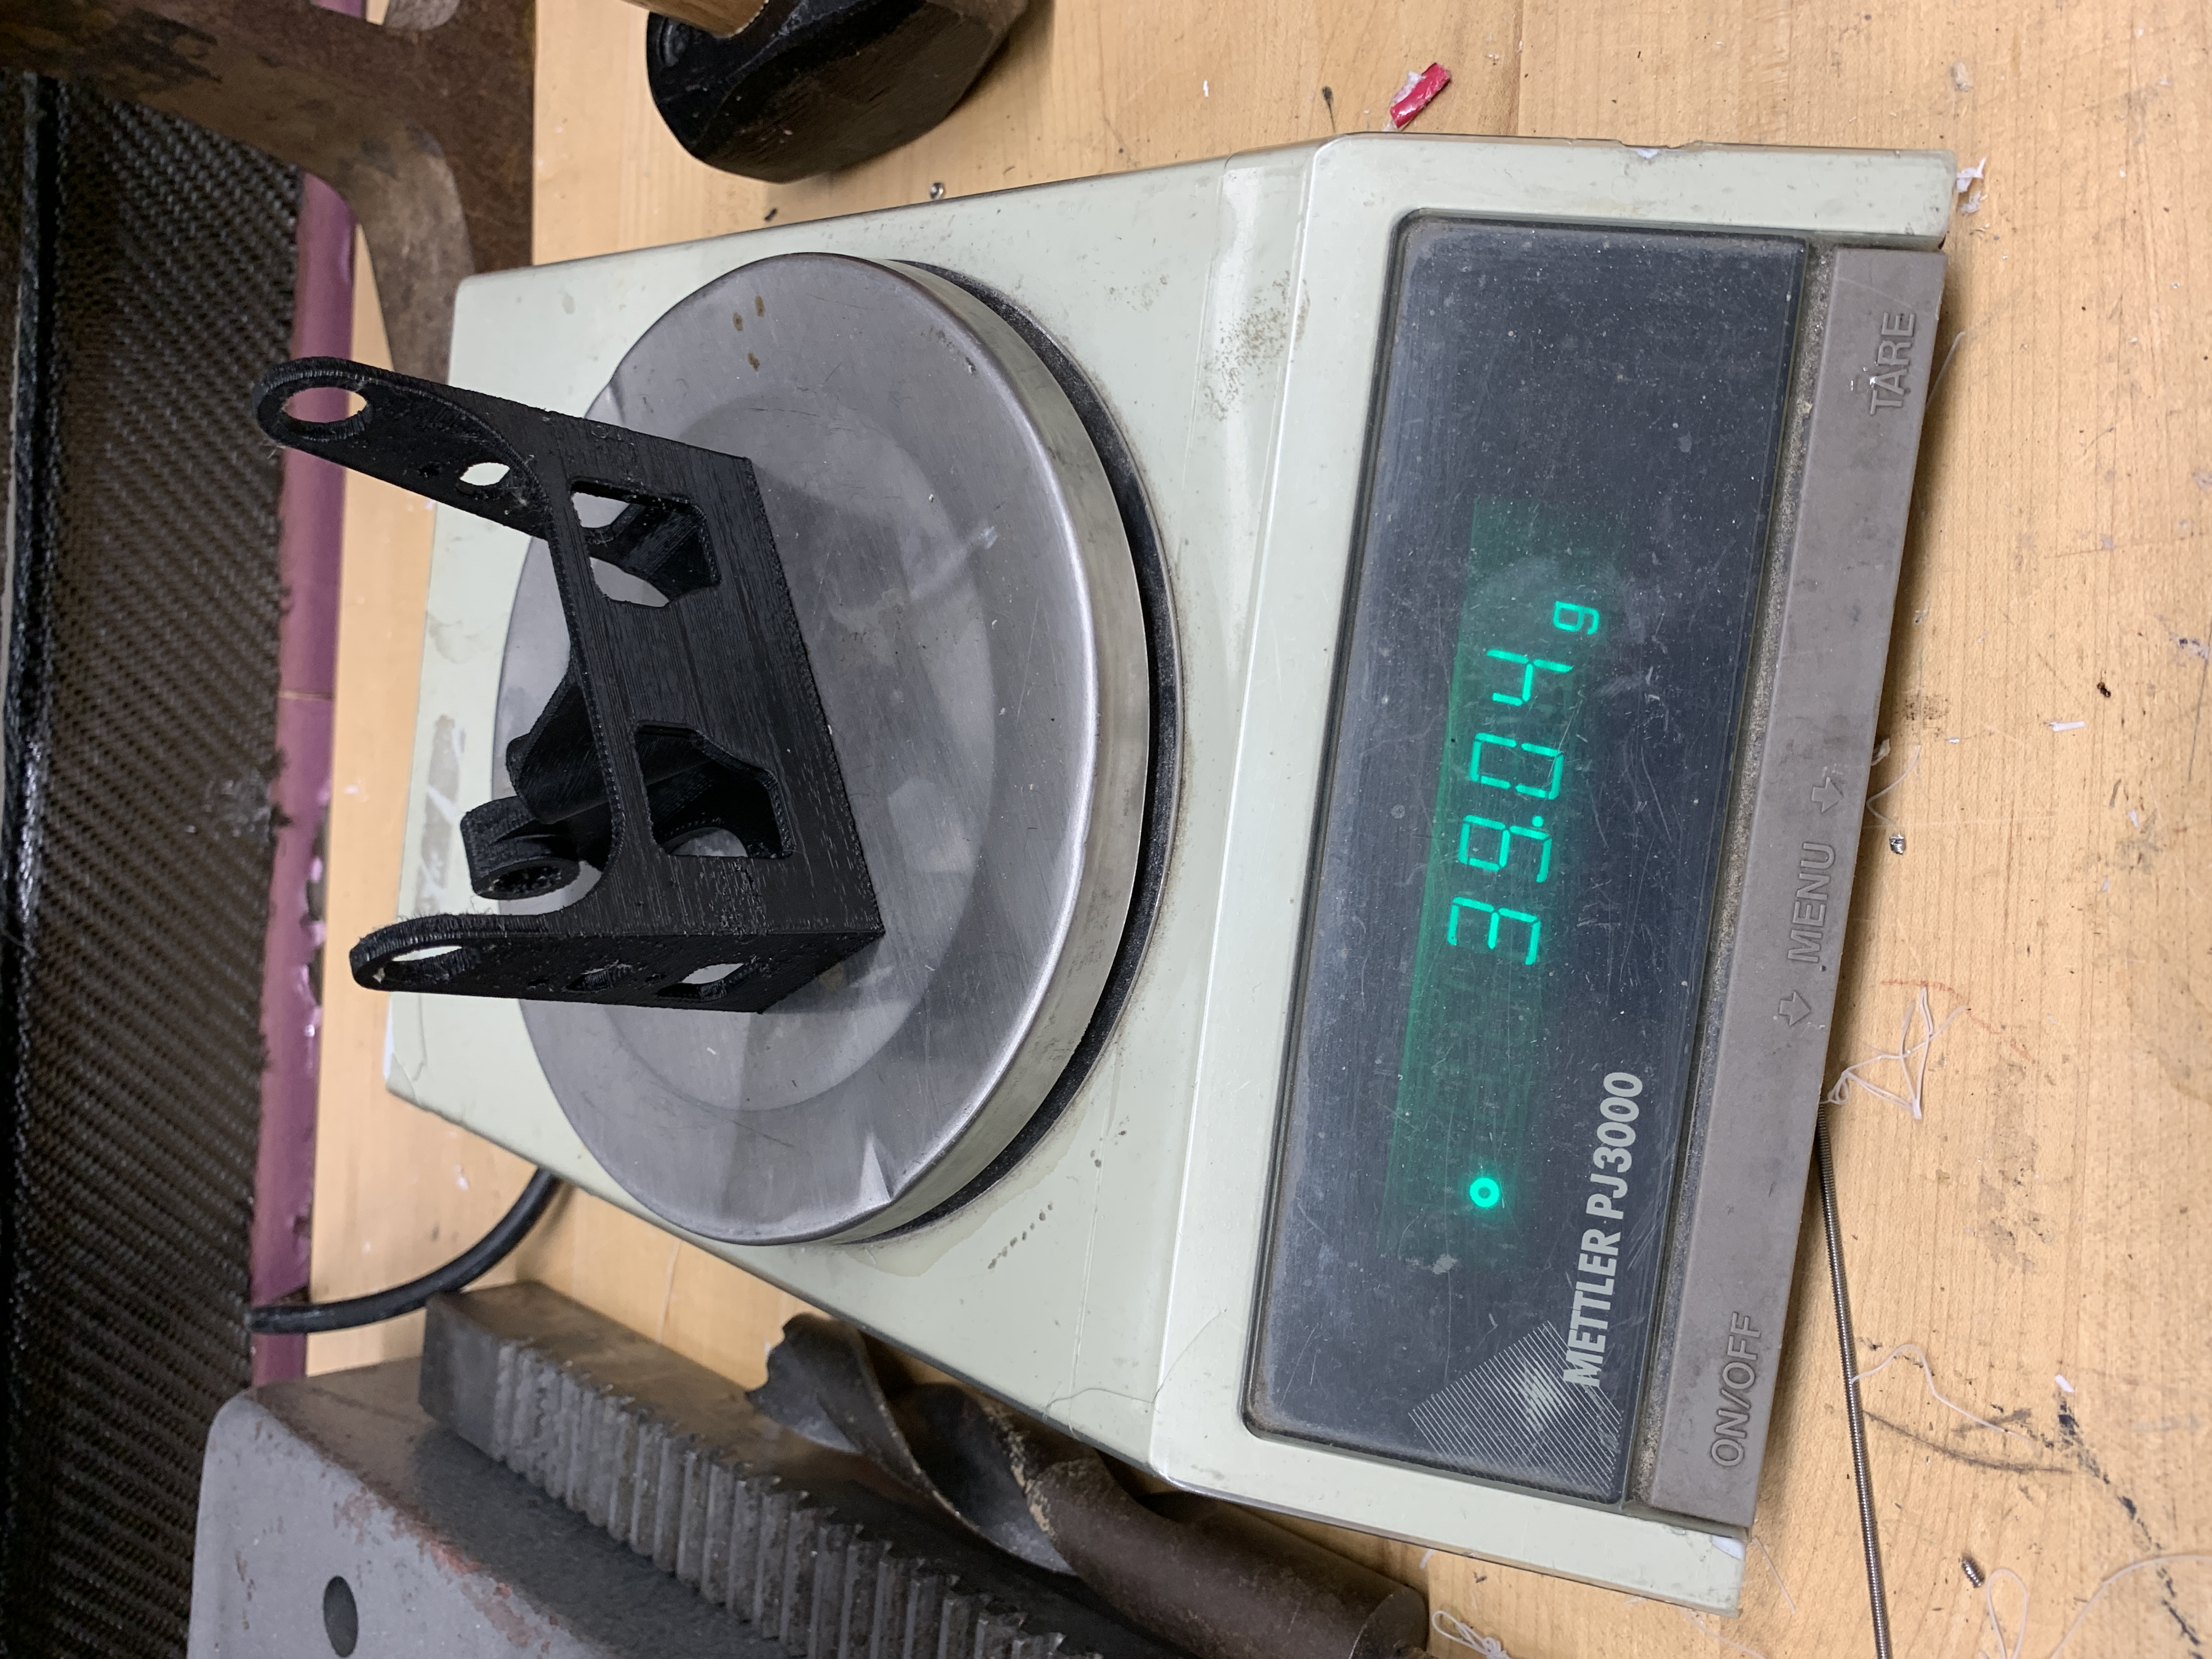
\includegraphics[width=0.95\textwidth]{Meetings/December/12-30-21/12-30-21_Hardware_Figure2 - Nathan Forrer.jpg}
  \caption{Our new intake was much lighter}
  \label{fig:123021_2}
\end{minipage}
\end{figure}

\begin{figure}[ht]
\centering
\begin{minipage}[b]{.48\textwidth}
  \centering
  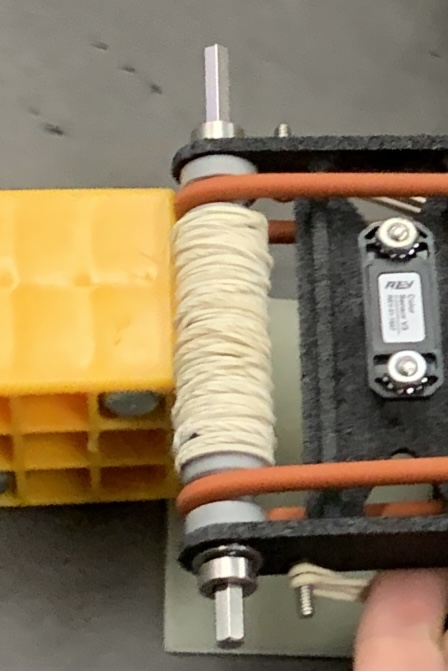
\includegraphics[width=0.95\textwidth]{Meetings/December/12-30-21/12-30-21_Hardware_Figure3 - Nathan Forrer.JPG}
  \caption{Covering the roller in rubber bands instead of surgical tubing}
  \label{fig:123021_3}
\end{minipage}%
\hfill%
\begin{minipage}[b]{.48\textwidth}
  \centering
  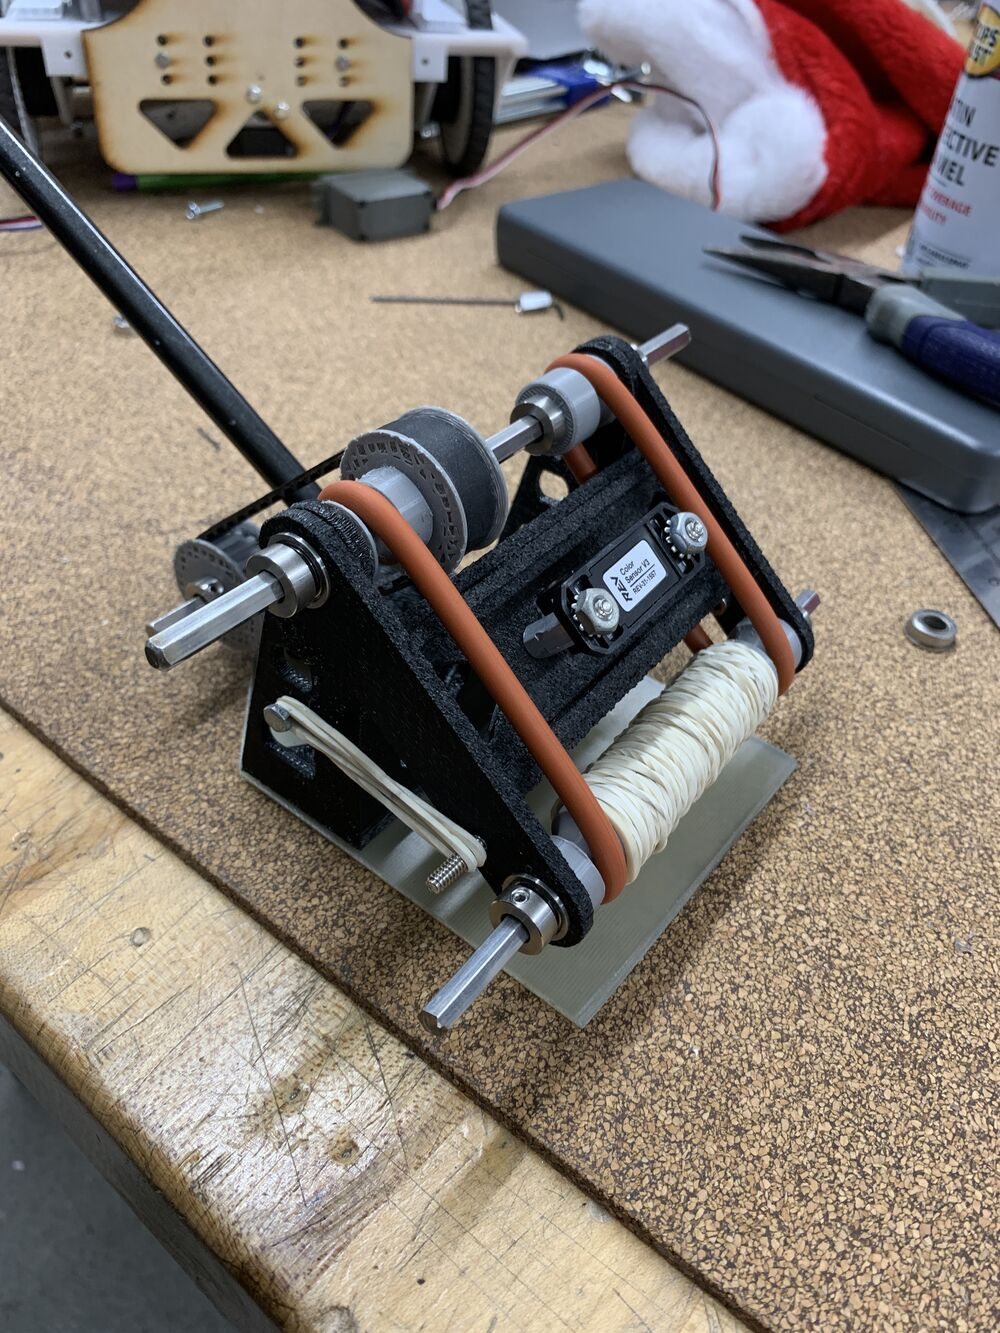
\includegraphics[width=0.95\textwidth]{Meetings/December/12-30-21/12-30-21_Hardware_Figure4 - Nathan Forrer.JPG}
  \caption{The completed intake}
  \label{fig:123021_4}
\end{minipage}
\end{figure}

\begin{figure}[ht]
\centering
\begin{minipage}[b]{.48\textwidth}
  \centering
  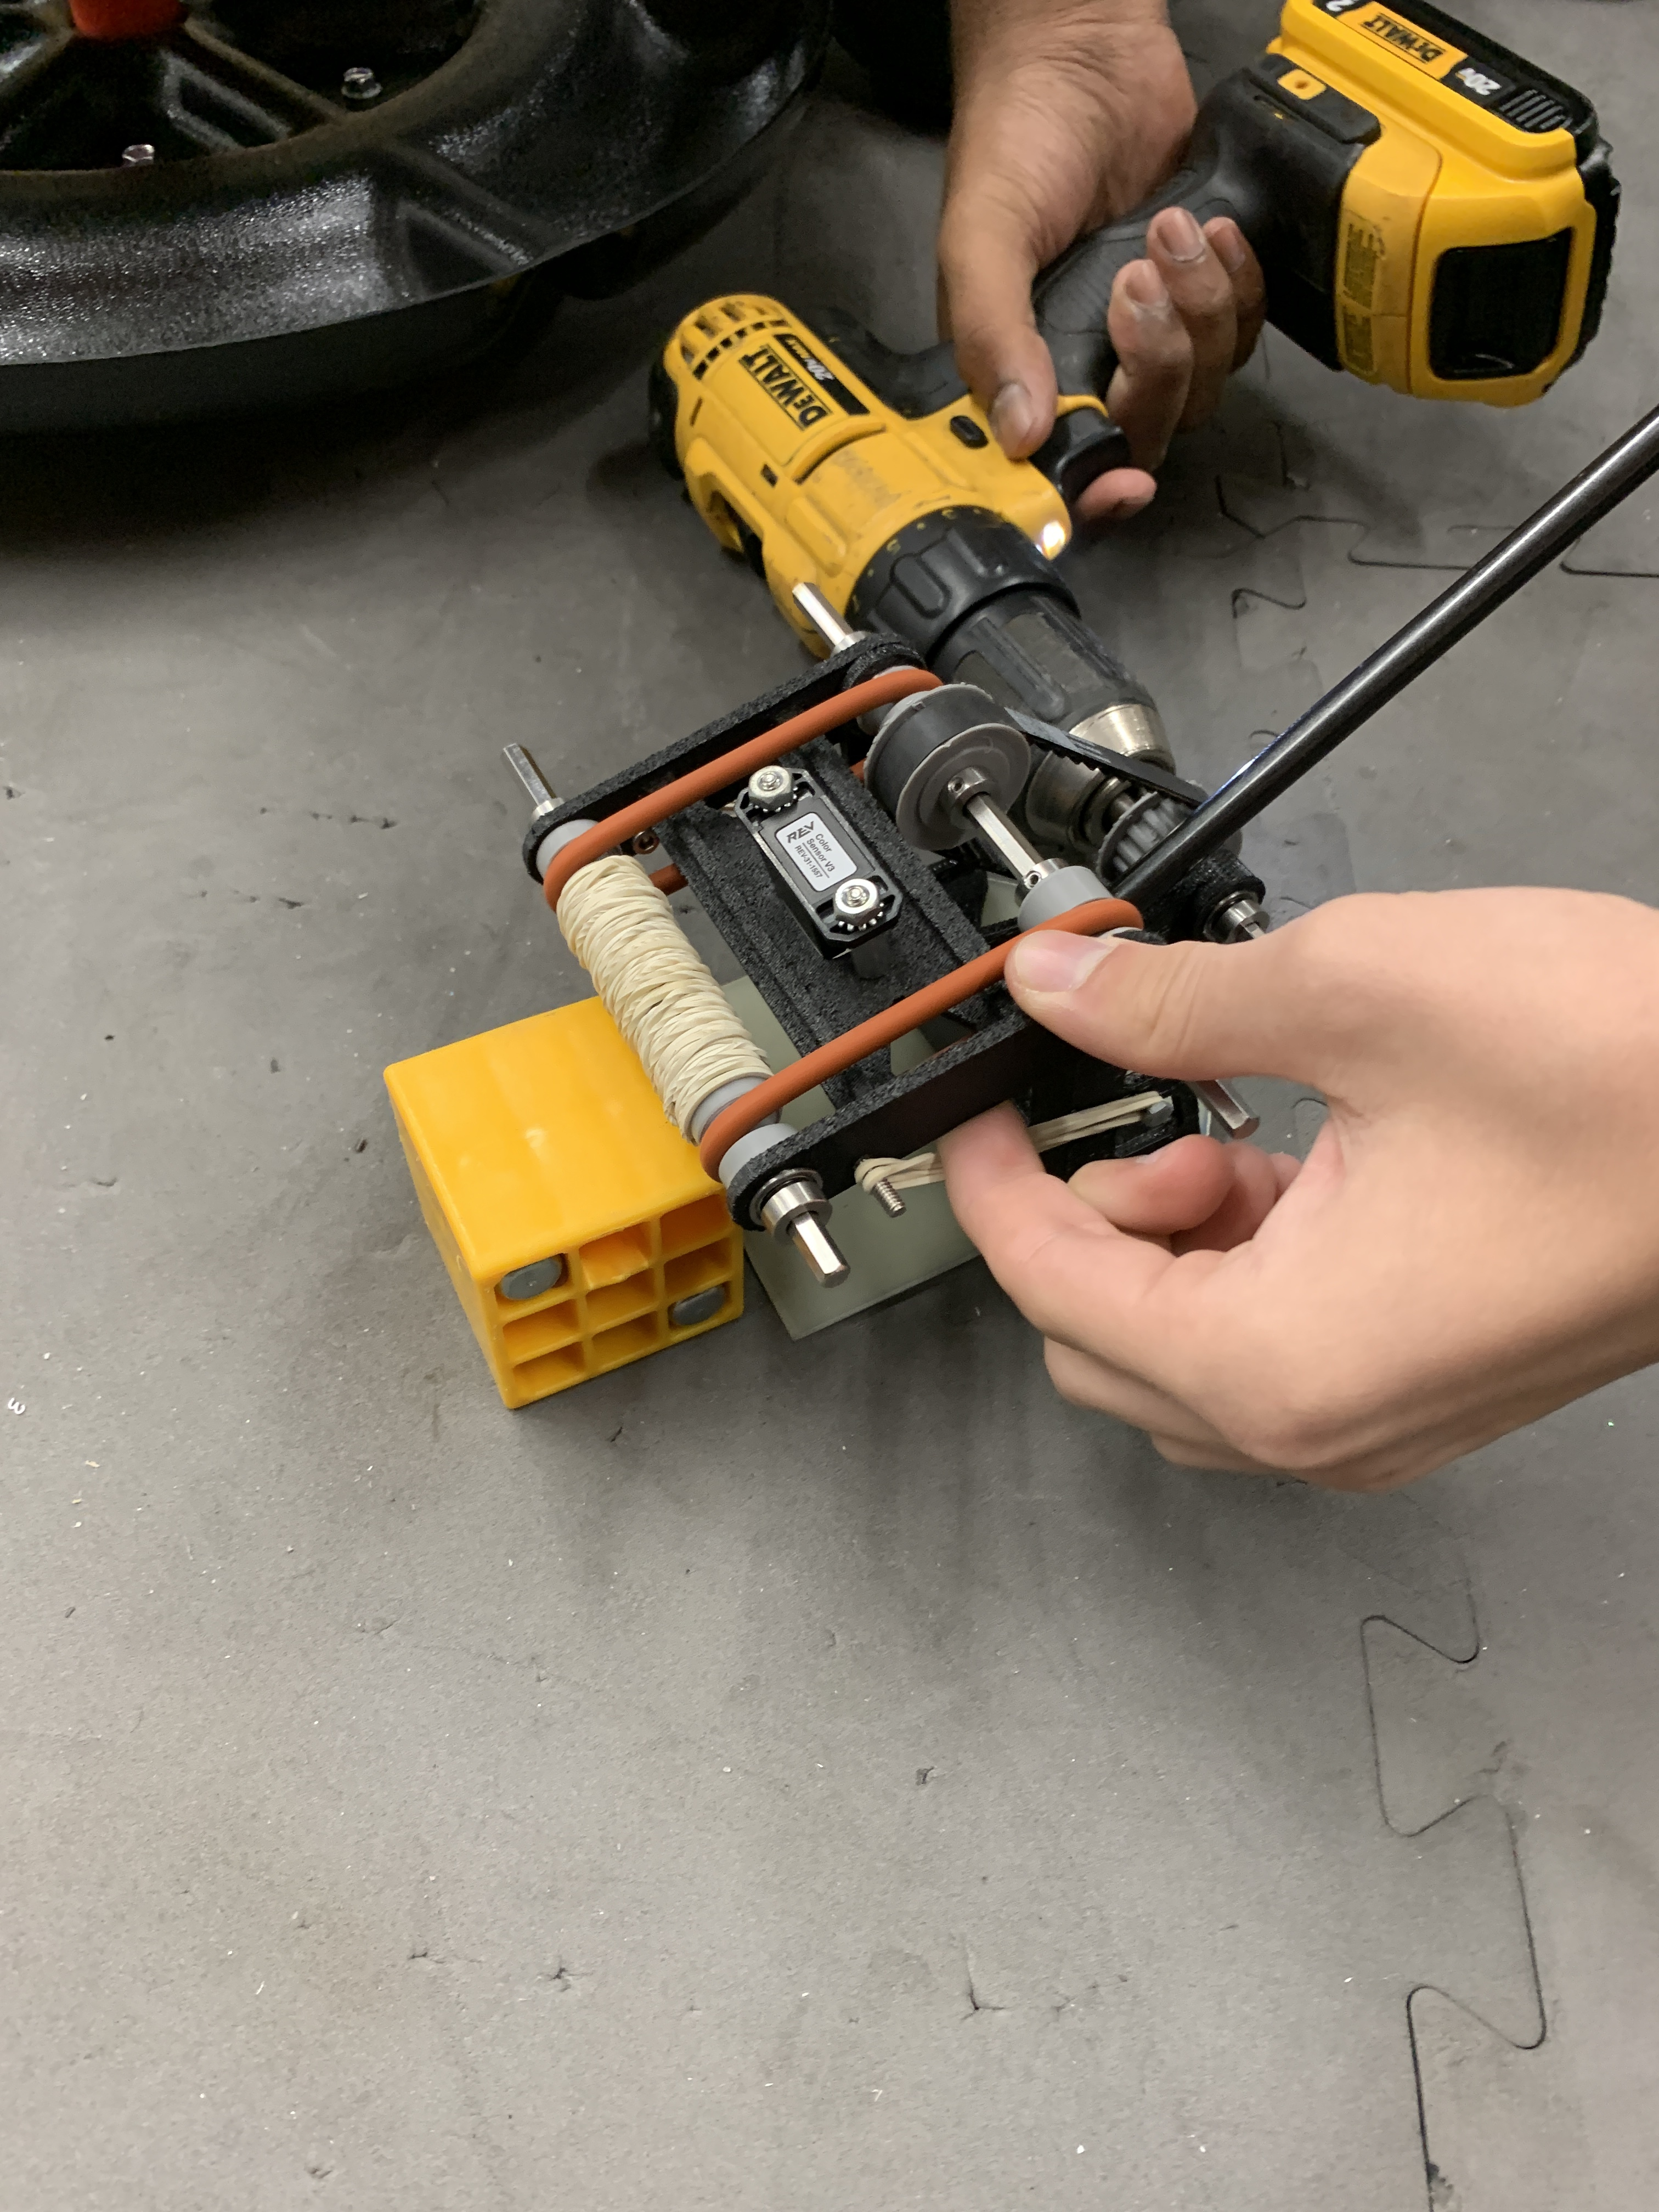
\includegraphics[width=0.95\textwidth, angle=0]{Meetings/December/12-30-21/12-30-21_Hardware_Figure5 - Nathan Forrer.JPG}
  \caption{Testing the intake using a drill as a "servo"}
  \label{fig:123021_5}
\end{minipage}%
\hfill%
\begin{minipage}[b]{.48\textwidth}
  \centering
  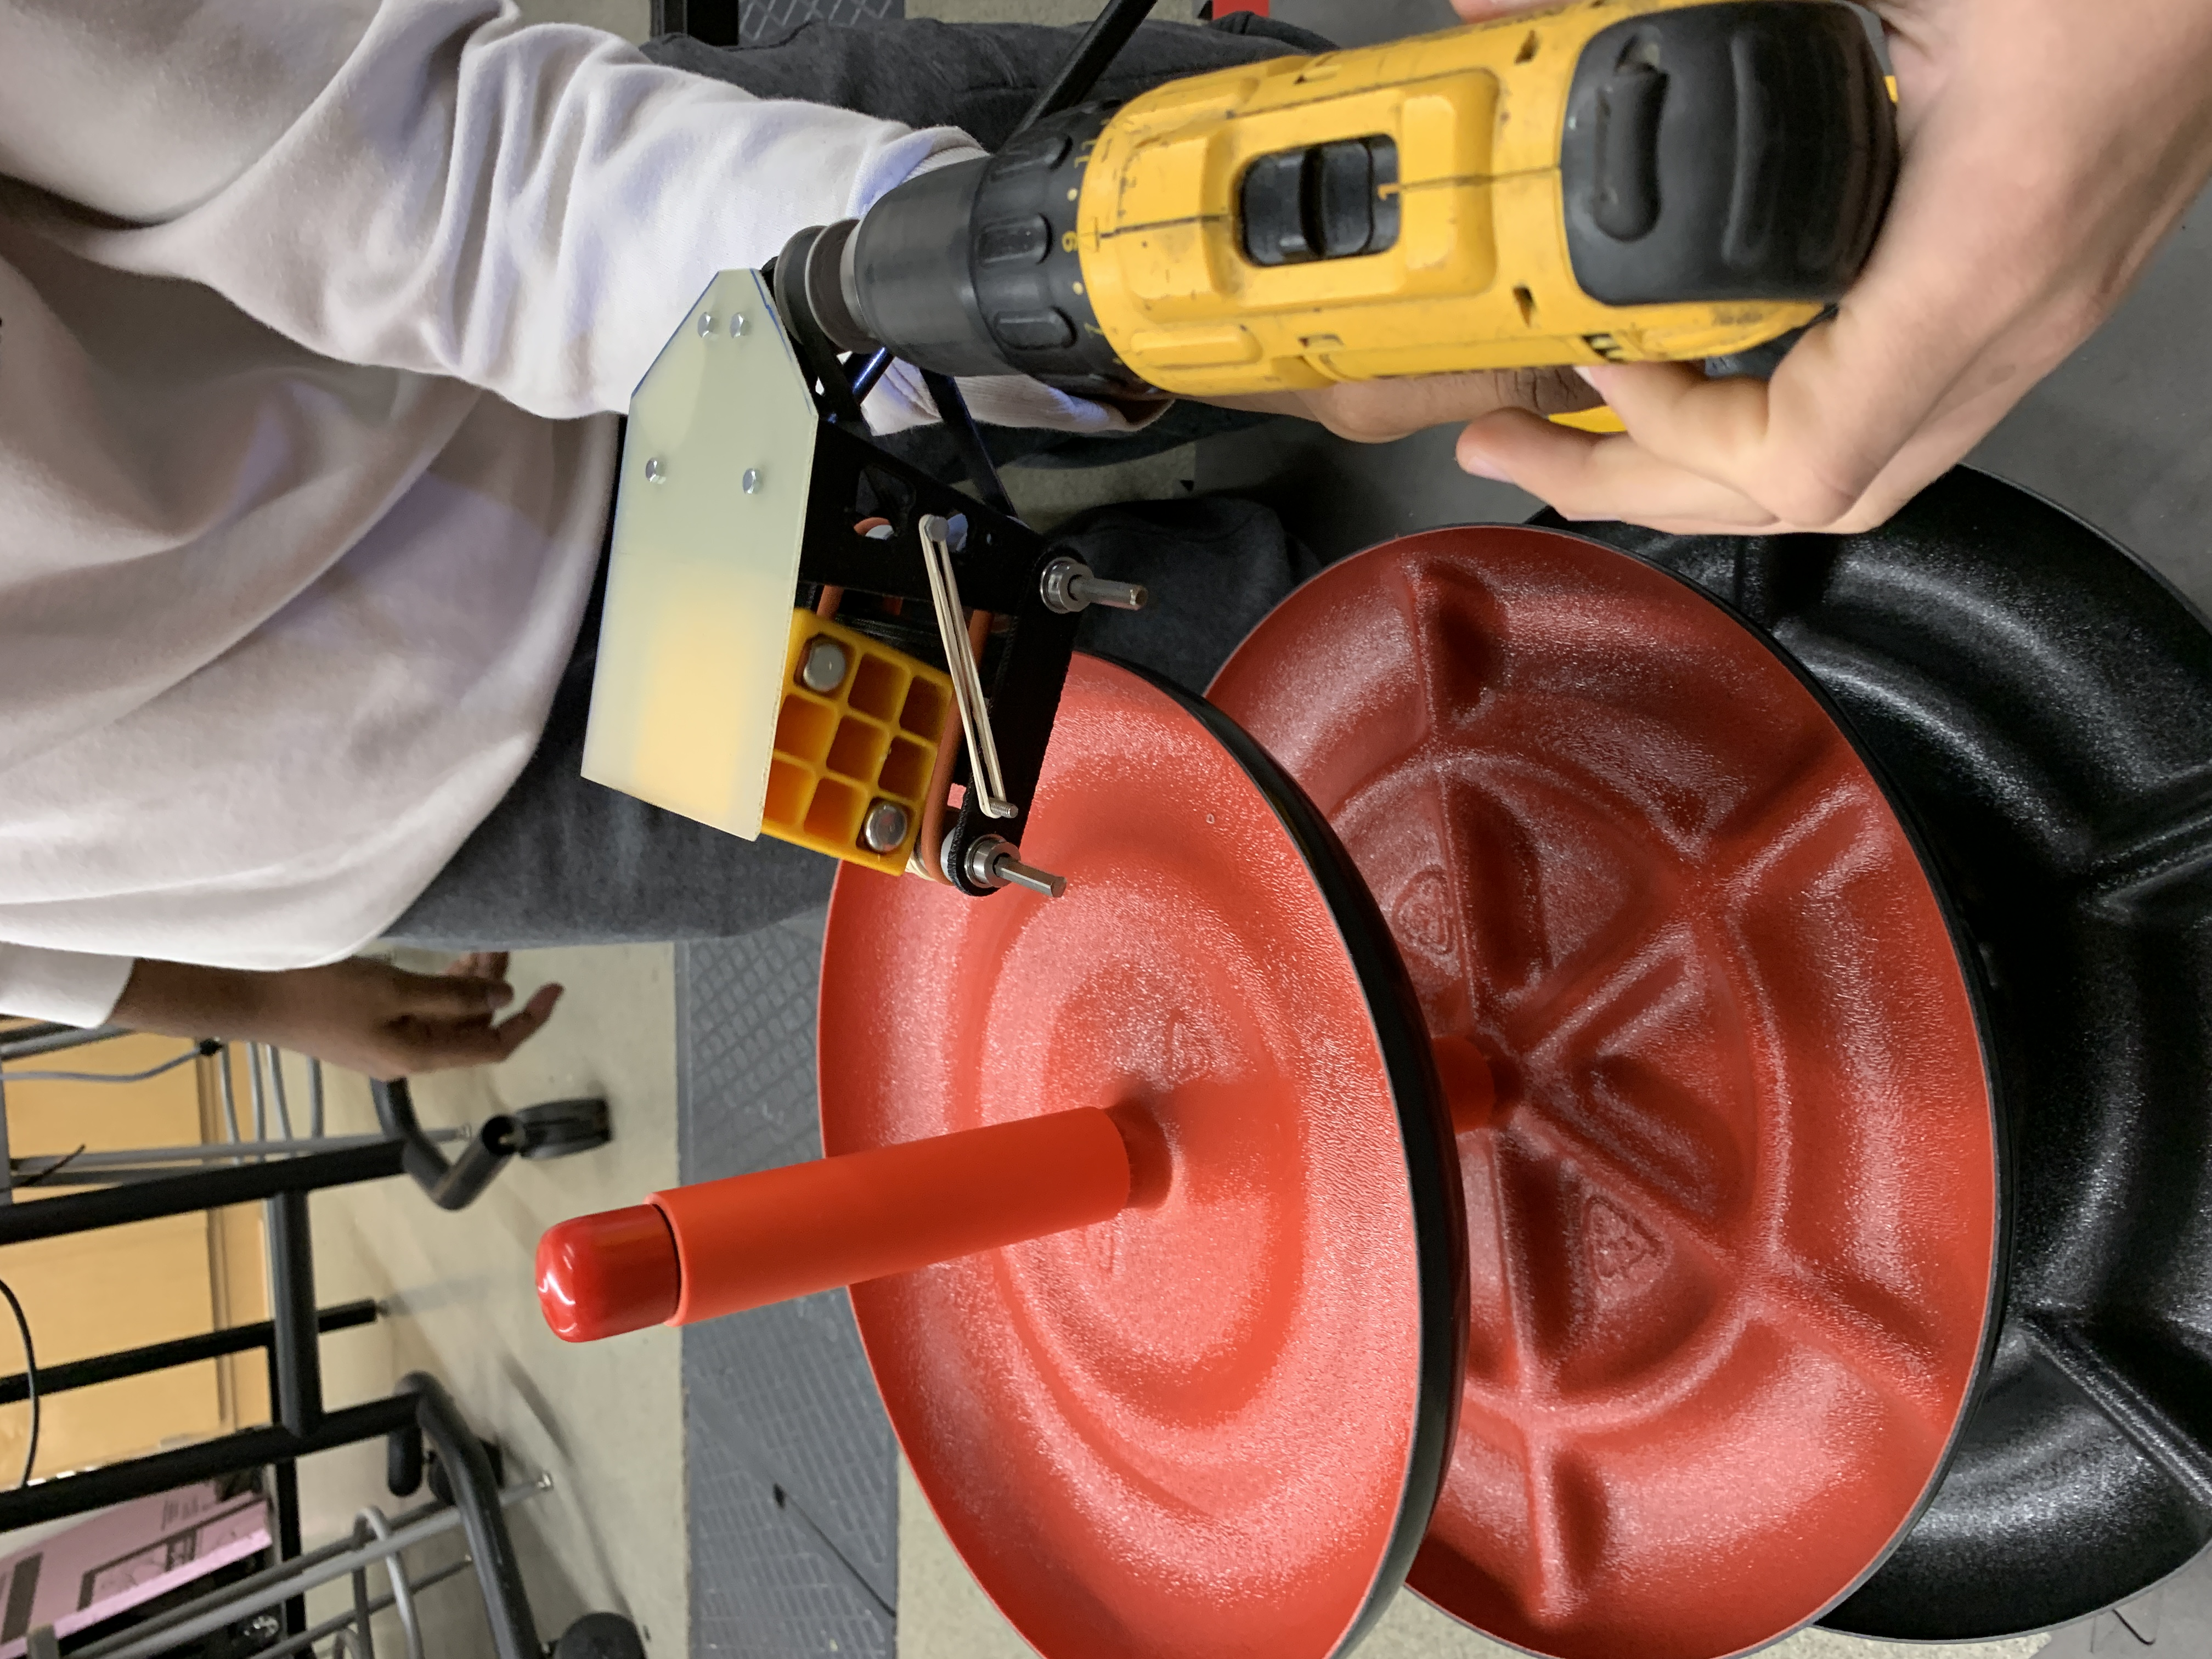
\includegraphics[width=0.95\textwidth]{Meetings/December/12-30-21/12-30-21_Hardware_Figure6 - Nathan Forrer.JPG}
  \caption{Element drop test}
  \label{fig:123021_6}
\end{minipage}
\end{figure}



\whatsnext{
\begin{itemize}
    \item Refine intake design to be usable at the upcoming competition on the 8th
\end{itemize} 
}

